\documentclass[sigchi, review]{acmart}

\usepackage{booktabs} % For formal tables


% Copyright
%\setcopyright{none}
\setcopyright{acmcopyright}
%\setcopyright{acmlicensed}
%\setcopyright{rightsretained}
%\setcopyright{usgov}
%\setcopyright{usgovmixed}
%\setcopyright{cagov}
%\setcopyright{licensedcagov}
%\setcopyright{cagovmixed}
%\setcopyright{licensedothergov}

%----------------------------------------------------------------------------------------------------
%
%	DOI, ISBN, CONFERENCE INFO
%
% DOI
%\acmDOI{10.475/123_4}

% ISBN
%\acmISBN{123-4567-24-567/08/06}

%Conference
%\acmConference[WOODSTOCK'97]{ACM Woodstock conference}{July 1997}{El
%  Paso, Texas USA}
%\acmYear{1997}
%\copyrightyear{2016}
%
%\acmPrice{15.00}

%----------------------------------------------------------------------------------------------------
%
%	TITLE
%
\begin{document}
\title{A Clean Template for SIGCHI Papers}
%\titlenote{Produces the permission block, and
%  copyright information}
%\subtitle{Extended Abstract}
%\subtitlenote{The full version of the author's guide is available as
%  \texttt{acmart.pdf} document}

%----------------------------------------------------------------------------------------------------
%
%	EXEMPLAR AUTHORS
%
\author{Anonymous for Review}

%\author{Ben Trovato}
%\authornote{Dr.~Trovato insisted his name be first.}
%\orcid{1234-5678-9012}
%\affiliation{%
%  \institution{Institute for Clarity in Documentation}
%  \streetaddress{P.O. Box 1212}
%  \city{Dublin}
%  \state{Ohio}
%  \postcode{43017-6221}
%}
%\email{trovato@corporation.com}
%
%\author{G.K.M. Tobin}
%\authornote{The secretary disavows any knowledge of this author's actions.}
%\affiliation{%
%  \institution{Institute for Clarity in Documentation}
%  \streetaddress{P.O. Box 1212}
%  \city{Dublin}
%  \state{Ohio}
%  \postcode{43017-6221}
%}
%\email{webmaster@marysville-ohio.com}

% The default list of authors is too long for headers.
%\renewcommand{\shortauthors}{B. Trovato et al.}

%----------------------------------------------------------------------------------------------------
%
%	ABSTRACT
%
\begin{abstract}
This paper provides a sample of a \LaTeX\ document which conforms,
somewhat loosely, to the formatting guidelines for
ACM SIG Proceedings.
\end{abstract}

%----------------------------------------------------------------------------------------------------
%
%	CCS
%
% The code below should be generated by the tool at
% http://dl.acm.org/ccs.cfm
% Please copy and paste the code instead of the example below.
%
\begin{CCSXML}
<ccs2012>
<concept>
<concept_id>10003120.10003121</concept_id>
<concept_desc>Human-centered computing~Human computer interaction (HCI)</concept_desc>
<concept_significance>500</concept_significance>
</concept>
</ccs2012>
\end{CCSXML}

\ccsdesc[500]{Human-centered computing~Human computer interaction (HCI)}


\keywords{Update, Your, Keywords, Here}

%----------------------------------------------------------------------------------------------------
%
%	EXEMPLAR TEASER
%
\begin{teaserfigure}
  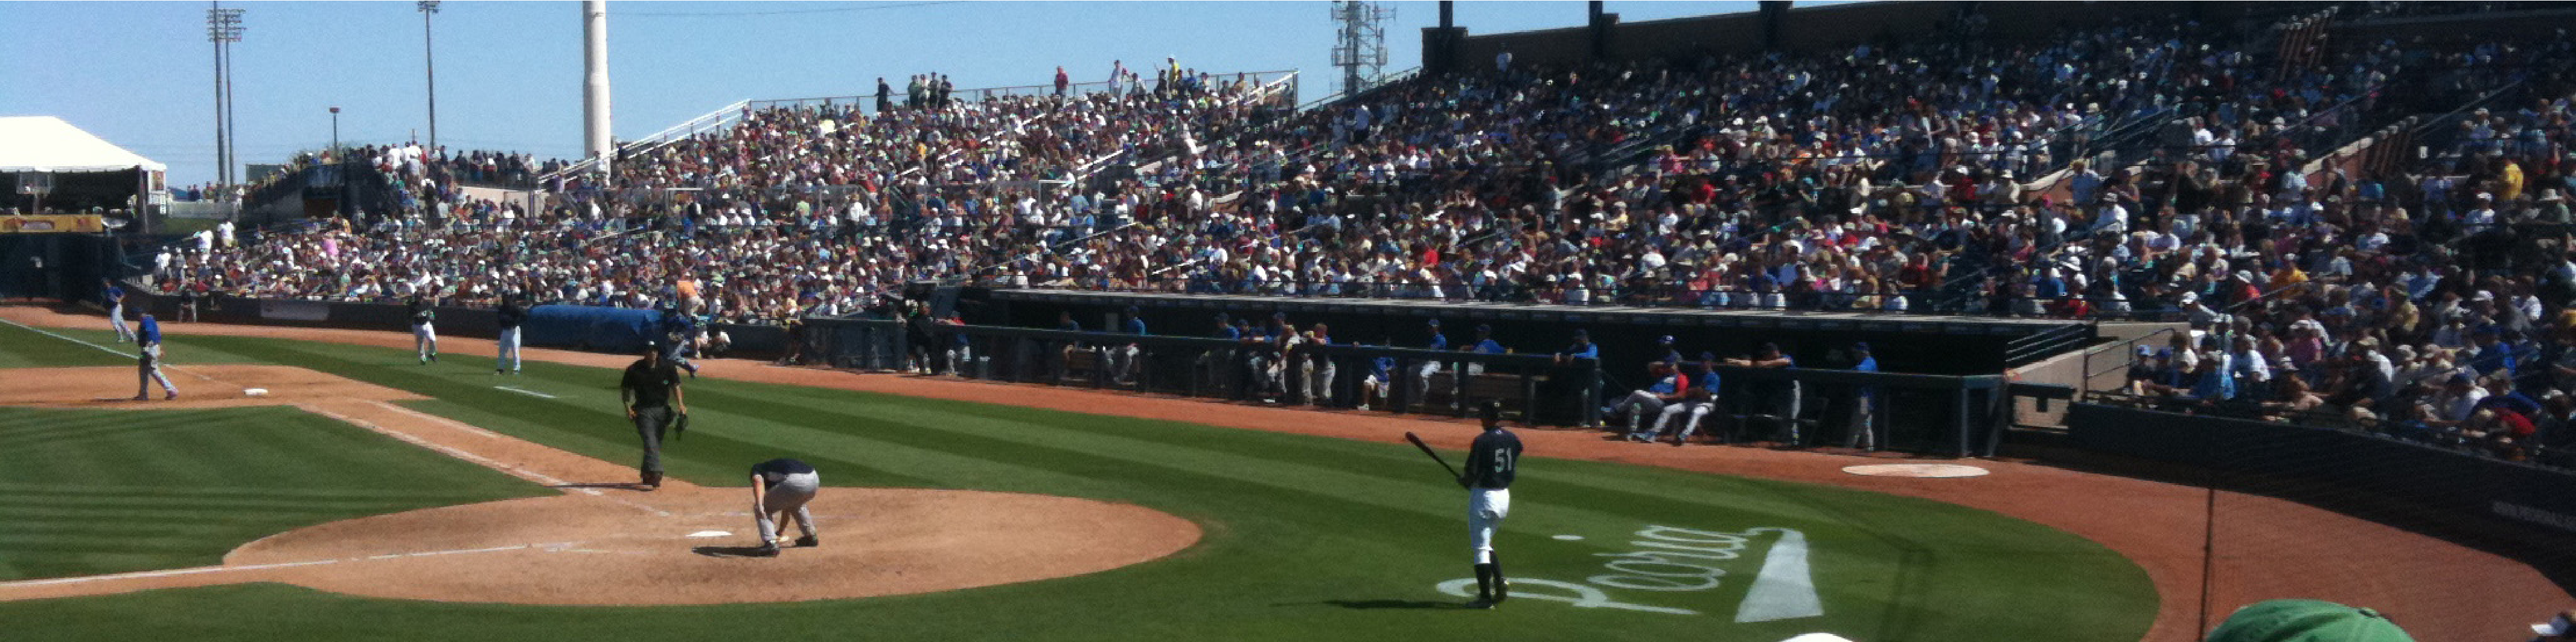
\includegraphics[width=\textwidth]{sampleteaser}
  \caption{This is a teaser}
  \label{fig:teaser}
\end{teaserfigure}

%----------------------------------------------------------------------------------------------------
%
%	THE PAPER
%	(See samplebody-conf for how to make stuff like tables, figures)
%
\maketitle

\section{Introduction}

\bibliographystyle{ACM-Reference-Format}
\bibliography{references}

\end{document}
